% !TeX program = lualatex
% !TeX encoding = utf8
% !TeX spellcheck = uk_UA
% !BIB program = bibler

\documentclass{beamer}
\usetheme{Electromagnetism}
\usepackage{Electromagnetism}
\usepackage{ocgx2}

%============================================================================
\title[Лекції електрики та магнетизму]{\huge\bfseries Енергія електромагнітного поля}
\subtitle{Лекції з електрики та магнетизму}
\author{Пономаренко С. М.}
%============================================================================
\graphicspath{{pictures/}}
\begin{document}
\begin{frame}[plain]
	\maketitle
\end{frame}



% ============================== Слайд ## ===================================
\begin{frame}{Локальні закони збереження}{}
	\begin{onlyenv}<1>
		\begin{block}{}\justifying
			Локальний закон збереження заряду стверджує, що заряд може перейти з одного місця в інше тільки за умови, що щось відбувається у просторі між ними. Щоб описати такий закон, нам потрібна не лише густина заряду $ \rho $, а й величина іншого сорту, саме вектор $ \vect{j} $, що задає швидкість потоку заряду через поверхню. При цьому потік пов'язаний з швидкістю зміни заряду рівнянням:
			\begin{equation*}
				\divg\vect{j} = -\parttime{\rho}.
			\end{equation*}

			Це сильніше формулювання закону збереження. Воно каже, що заряд зберігається особливим чином, зберігається \emph{локально}.

			\bigskip

			Збереження енергії, виявляється, також локальний процес. У світі існує не тільки густина енергії в даної області, а й вектор, що є швидкістю потоку енергії через поверхню.
		\end{block}
	\end{onlyenv}
	\begin{onlyenv}<2>
		\begin{columns}
			\begin{column}{0.5\linewidth}
				\begin{center}
					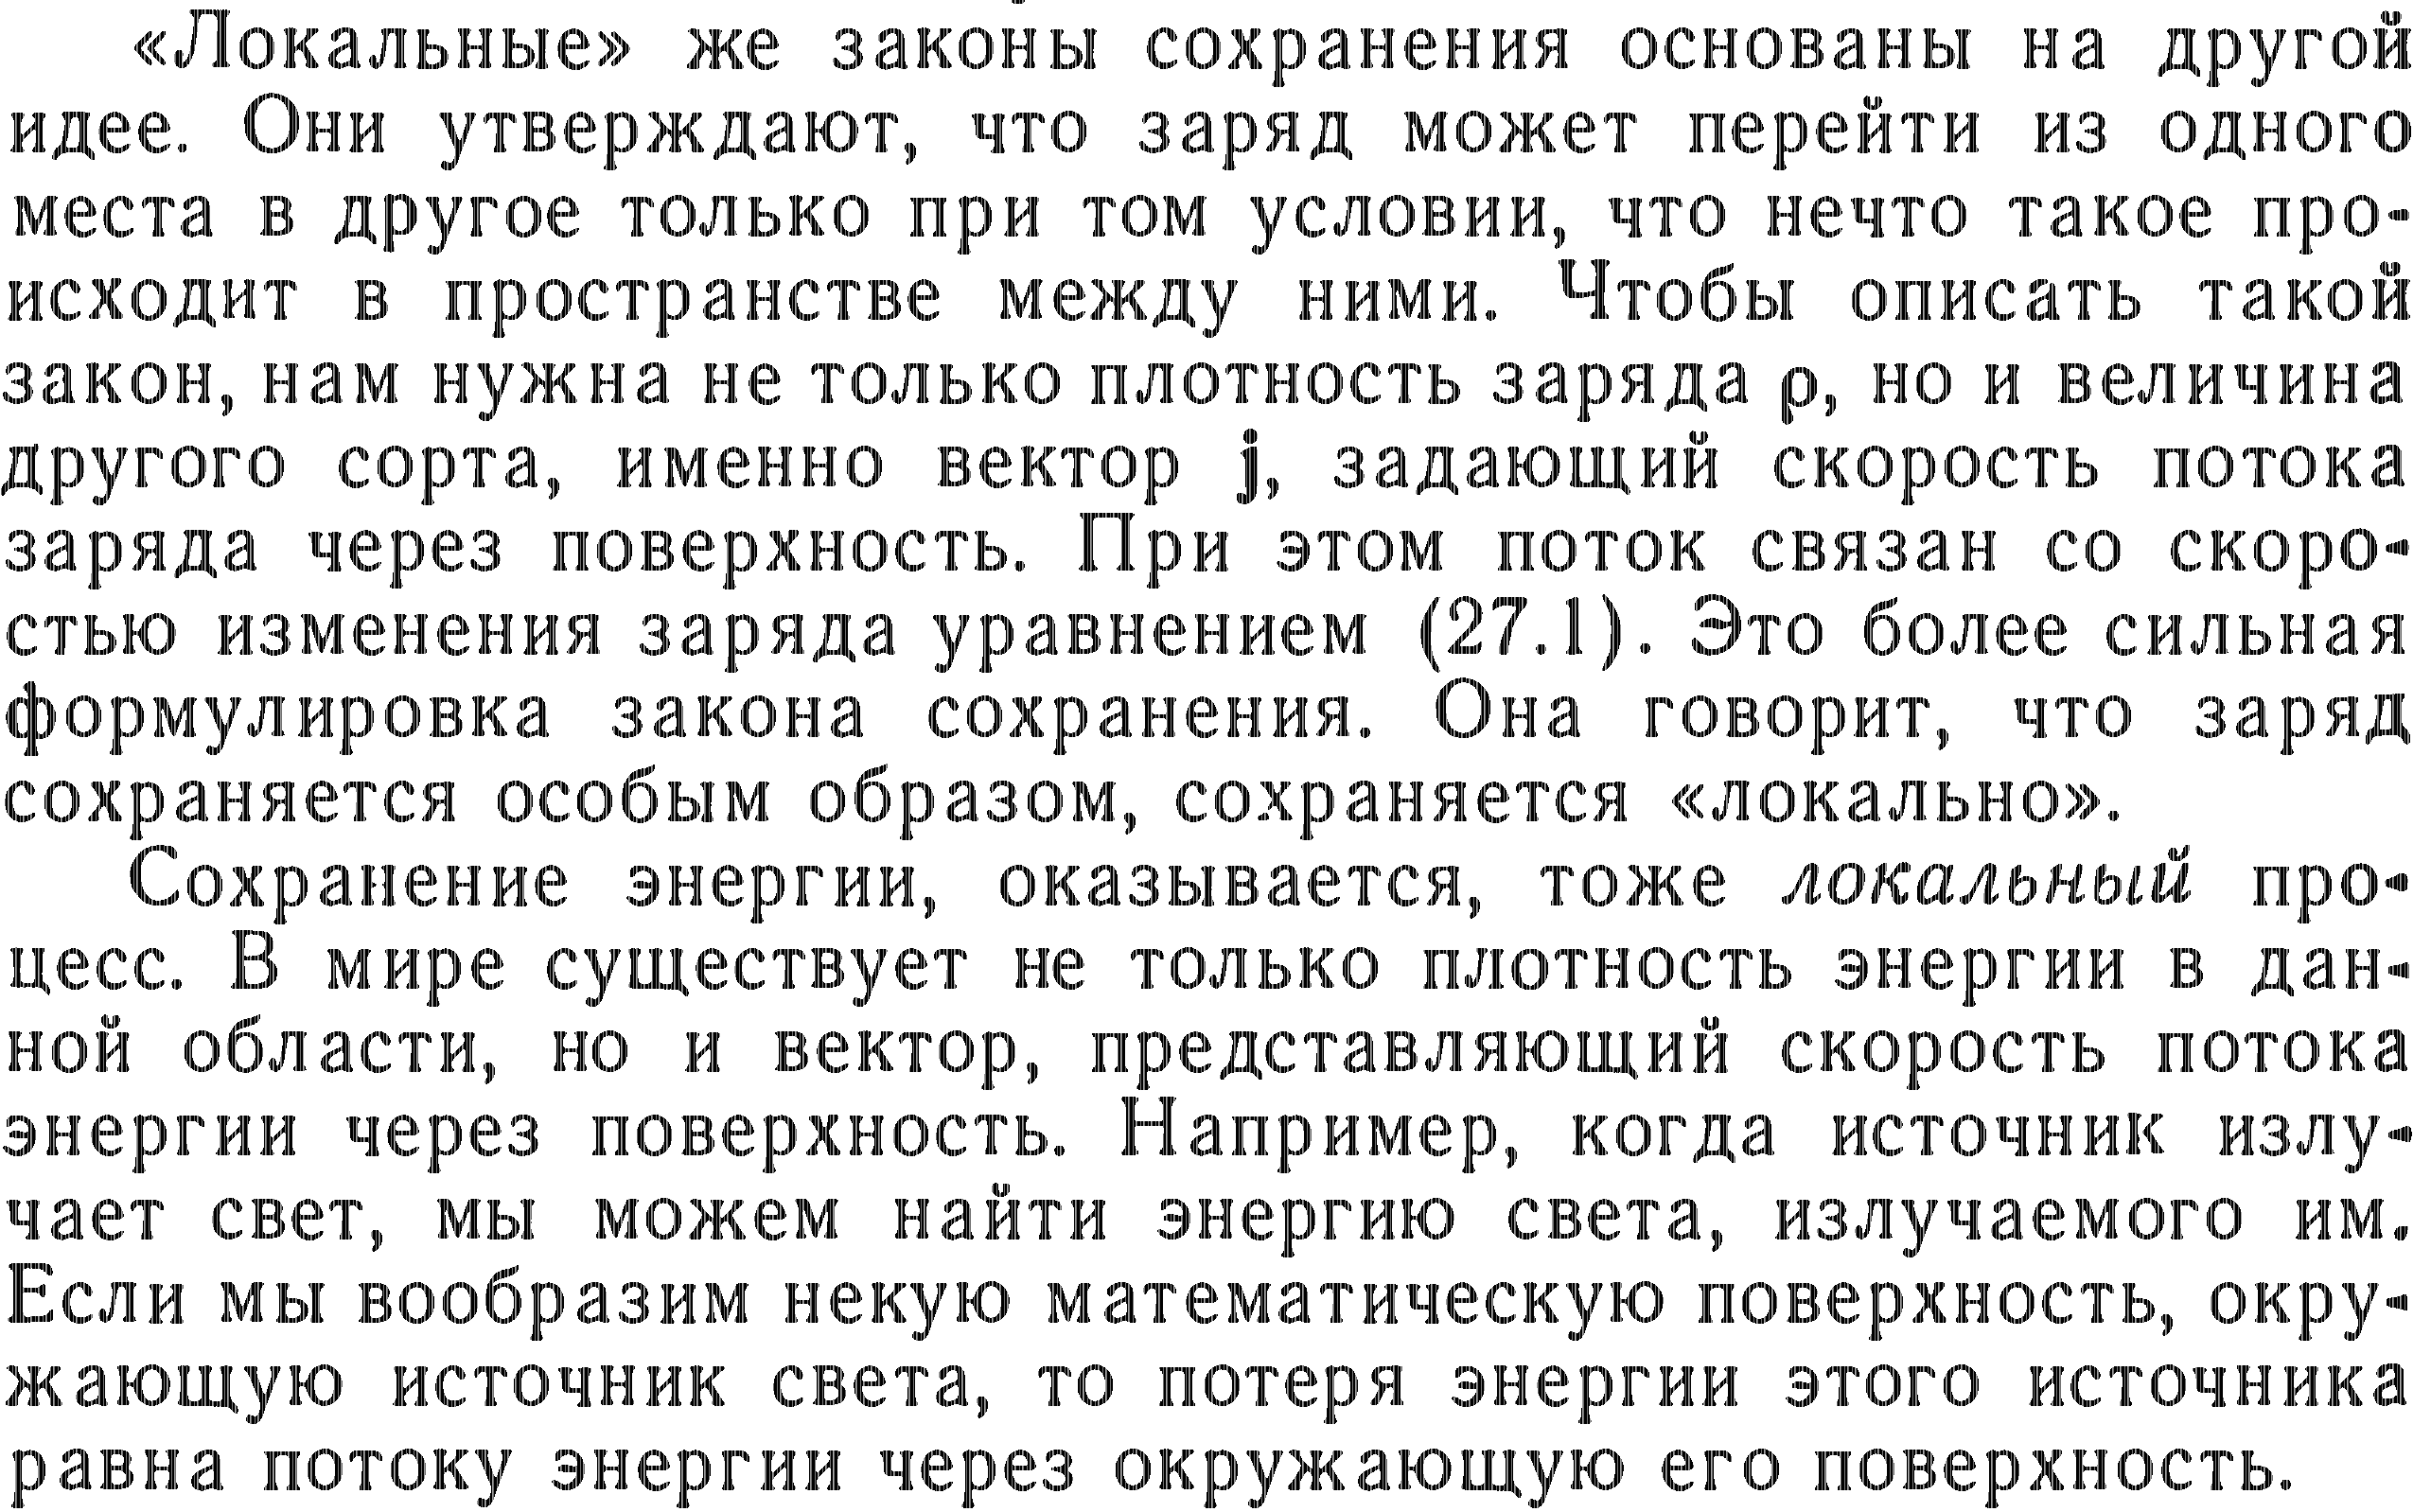
\includegraphics[width=\linewidth]{pictures/FML-local_Law}
				\end{center}
			\end{column}
			\begin{column}{0.5\linewidth}
				\begin{center}
					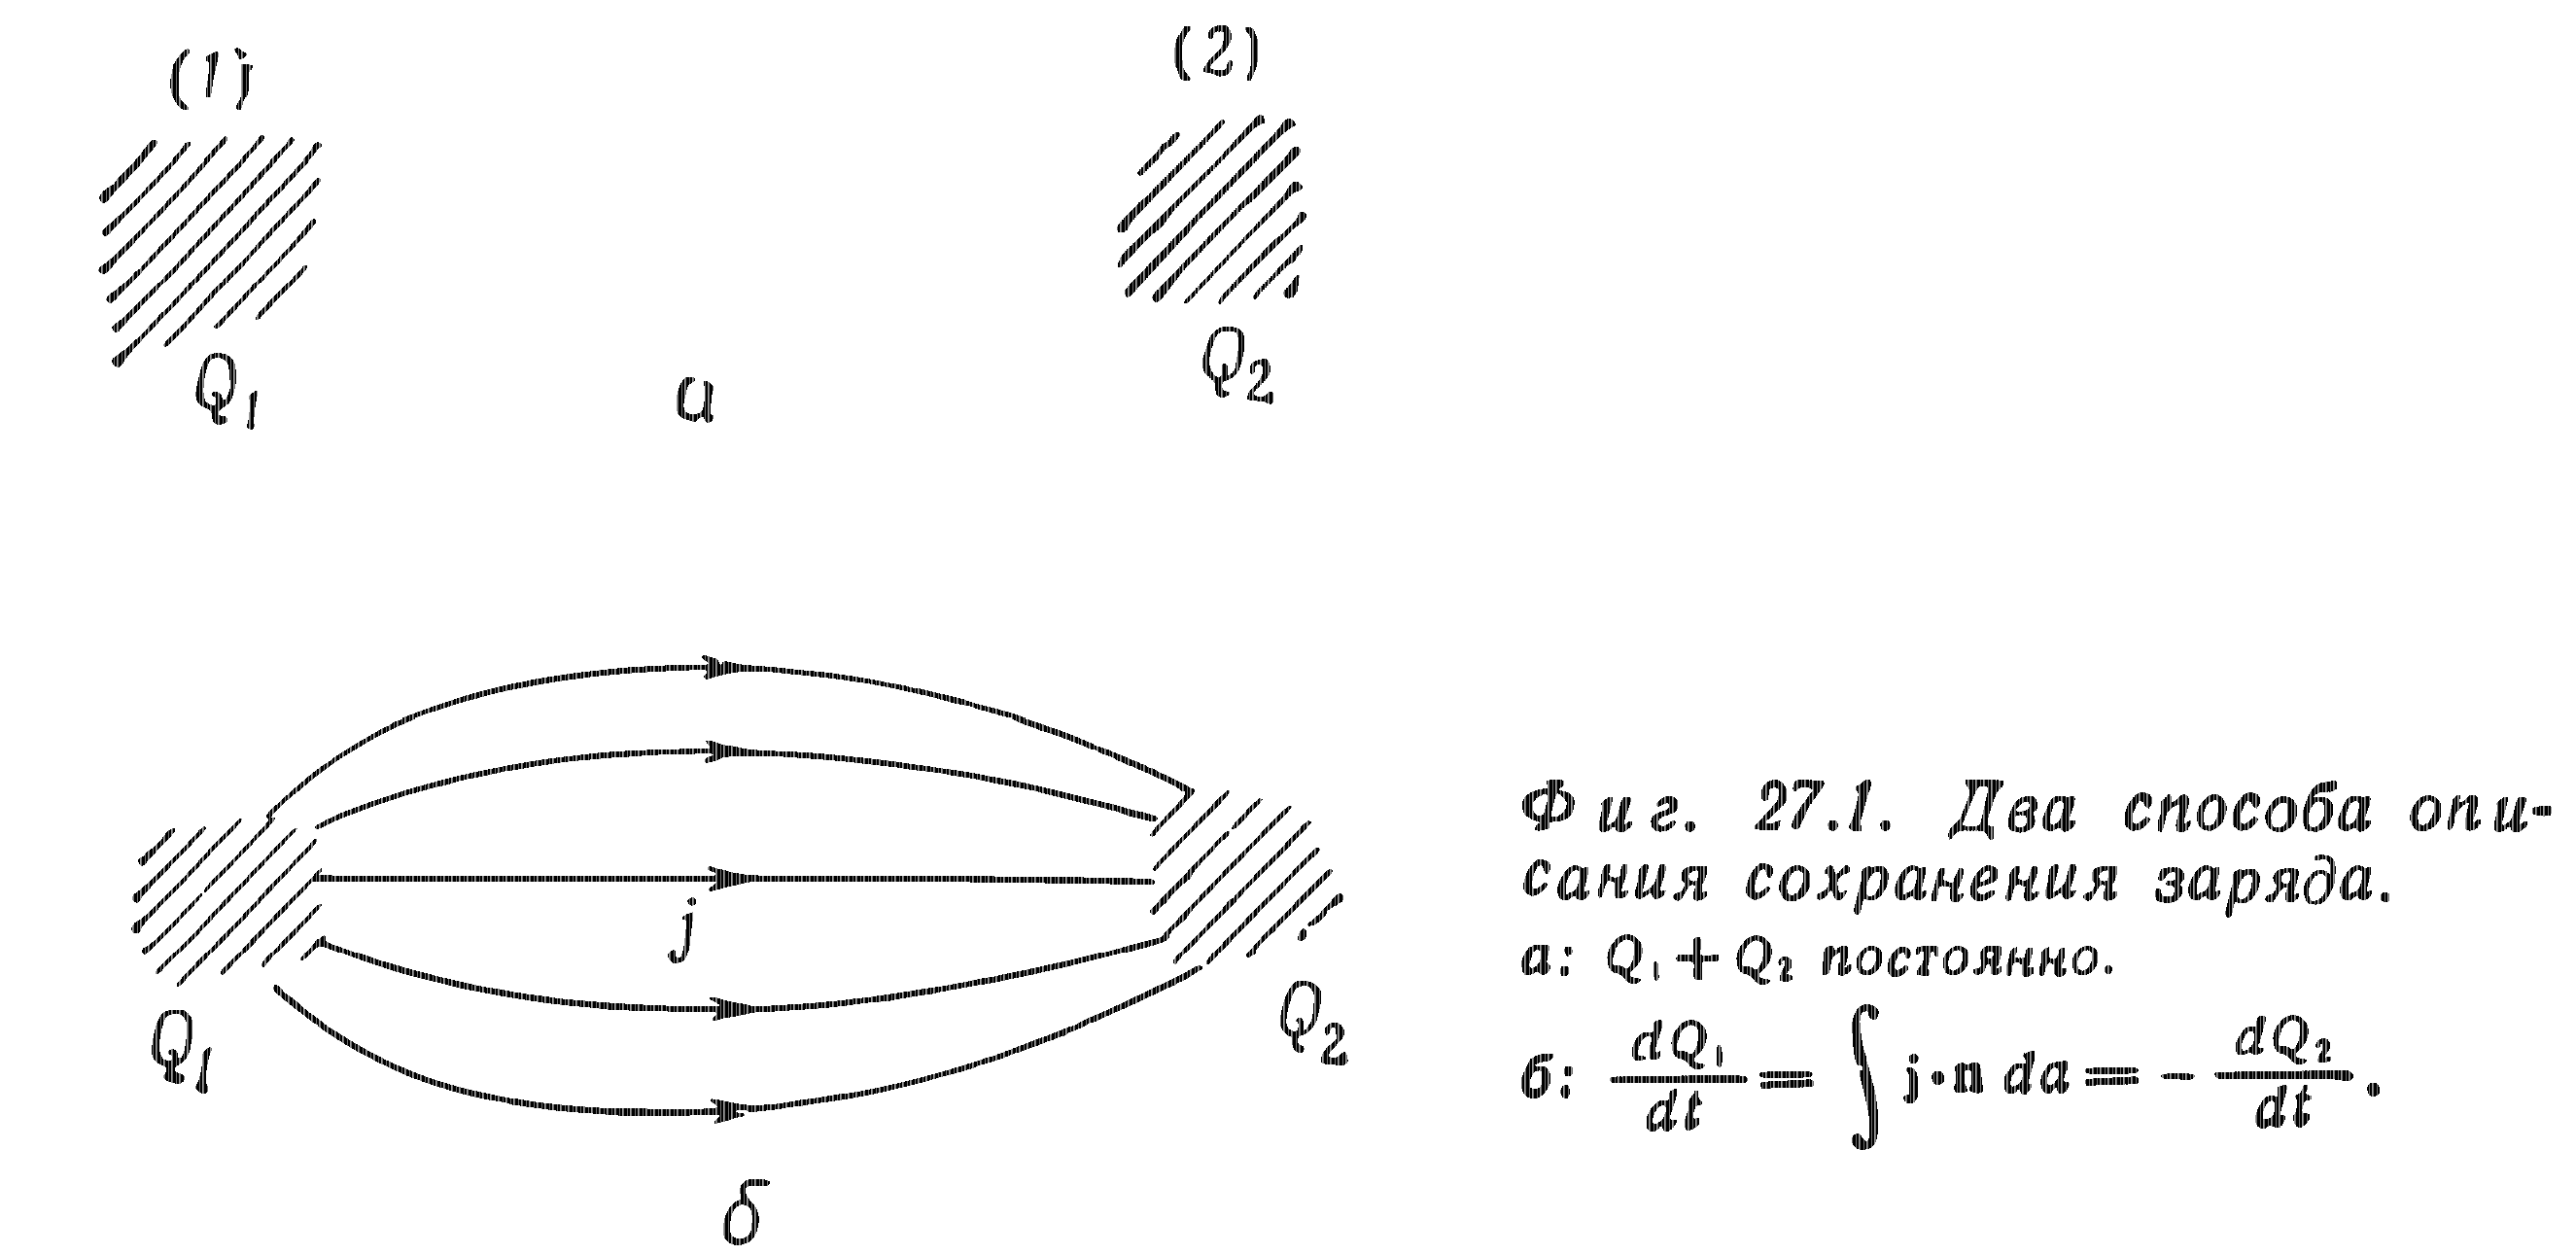
\includegraphics[width=\linewidth]{pictures/FML-local_Law-pic}
				\end{center}
			\end{column}
		\end{columns}
	\end{onlyenv}
\end{frame}
% ===========================================================================






% ============================== Слайд ## ===================================
\begin{frame}{Закон збереження енергії}{}
	\begin{center}
		\begin{equation*}\small
			(\text{Зменшення енергії в об'ємі}) = (\text{виконання роботи}) + (\text{потік на зовні})
		\end{equation*}
	\end{center}
	\begin{columns}
		\begin{column}{0.3\linewidth}
			\begin{center}
				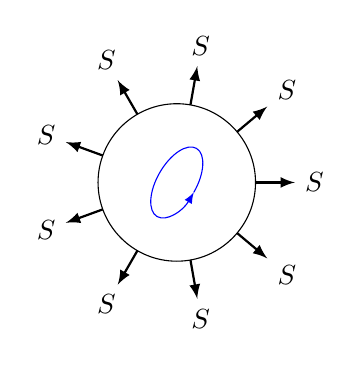
\begin{tikzpicture}
					\draw[] (0,0) circle (1);
					\foreach \p in {0,40,...,320} {
							\draw[-latex, thick]  (0,0) ++(\p:1) -- ++(\p:0.5) node[anchor={\p-180}] {$\vect{S}$};
						}
					\draw [-latex,  rotate=-30, blue] (0.25,0) arc [start angle=0, end angle=360, x radius=0.25cm, y radius=0.5cm] ;
				\end{tikzpicture}
			\end{center}
		\end{column}
		\begin{column}{0.6\linewidth}\small
			\begin{equation*}
				-\frac{\partial W}{\partial t} =  Q + \oiint\limits_S \vect{S} d\vect{S}
			\end{equation*}

			$ W = \iiint\limits_V w dV$ --- енергія поля, \\
			$ Q = \iiint\limits_V \vect{j}\cdot\vect{E} dV$ --- робота, що витрачається полем на <<штовхання>> зарядів (роботу виконує лише електричне поле), \\
			$ \vect{S} $ --- вектор густини потоку енергії.

			В диференціальній формі
			\begin{equation*}
				-\frac{\partial w}{\partial t} =  \vect{j}\cdot\vect{E} + \vect{\nabla}\cdot\vect{S}
			\end{equation*}
		\end{column}
	\end{columns}

\end{frame}
% ===========================================================================



% ============================== Слайд ## ===================================
\begin{frame}{Виведення}{}
	\begin{equation*}
		\vect{j}\cdot\vect{E} = -\frac{\partial w}{\partial t} -   \vect{\nabla}\cdot\vect{S}
	\end{equation*}

	\begin{equation*}
		\vect{j} = \frac{c}{4\pi} \rot\Hfield - \frac1c \parttime{\Dfield}
	\end{equation*}

	\begin{equation*}
		\vect{j}\cdot\vect{E} =  \frac{c}{4\pi}  \Efield\cdot \rot\Hfield - \frac1{4\pi}  \Efield \parttime{\Dfield}
	\end{equation*}

	\begin{equation*}
		\divg[\Efield\times\Hfield] = \Hfield\cdot \rot\Efield - \Efield\cdot \rot\Hfield
	\end{equation*}

	\begin{equation*}
		\vect{j}\cdot\vect{E} =  - \divg\left(\frac{c}{4\pi}[\Efield\times\Hfield]\right) + \frac{c}{4\pi}  \Hfield\cdot \rot\Efield  -   \parttime{} \left( \frac1{8\pi}\epsilon\Efield^2\right)
	\end{equation*}

	\begin{equation*}
		\vect{j}\cdot\vect{E} =  - \divg\left(\frac{c}{4\pi}[\Efield\times\Hfield]\right) - \frac{1}{4\pi}  \Hfield\cdot \parttime{\Bfield}  -   \parttime{} \left( \frac1{8\pi}\epsilon\Efield^2\right)
	\end{equation*}

	\begin{equation*}
		\vect{j}\cdot\vect{E} =  -  \parttime{} \left( \frac1{8\pi}\epsilon\Efield^2 + \frac1{8\pi}\mu\Hfield^2 \right)
		- \divg\left(\frac{c}{4\pi}[\Efield\times\Hfield]\right)
	\end{equation*}

\end{frame}
% ===========================================================================




% ============================== Слайд ## ===================================
\begin{frame}{Вектор Пойнтінга}{}

	Вектор густини потоку енергії (вектор Пойнтінга)
	\begin{equation*}
		\vect{S} = \frac{c}{4\pi}[\Efield\times\Hfield], \quad [S] = \frac{\text{ерг}}{\text{см}^2 \cdot \text{с}}\, (\text{СГС}), [S] = \frac{\text{Вт}}{\text{м}^2}\, (\text{SI})
	\end{equation*}

	Густина енергії
	\begin{equation*}
		w = \frac{\Efield\cdot\Dfield}{8\pi} + \frac{\Bfield\cdot\Hfield}{8\pi}, \quad [w] = \frac{\text{ерг}}{\text{см}^2}\, (\text{СГС}), [w] = \frac{\text{Дж}}{\text{м}^3}\, (\text{SI})
	\end{equation*}

	\begin{block}{}\justifying\scriptsize
		З виразу для густини енергії ми бачимо, що вона є сумою «електричної» та «магнітної» густин енергій, які у точності дорівнюють виразам, отриманим нами у статиці. Крім того, ми отримали вираз для вектора потоку енергії електромагнітного поля. Цей новий вектор $ \vect{S} = \frac{c}{4\pi}[\Efield\times\Hfield] $ по імені свого першовідкривача називається <<вектором Пойнтинга». Він каже нам про напрямок і швидкість, з якою енергія рухається у просторі.
	\end{block}

\end{frame}
% ===========================================================================




% ============================== Слайд ## ===================================
\begin{frame}{Невизначеність енергії поля}{}
	Якщо покласти потік енергії рівним $ \vect{S}' = \vect{S} + \rot\vect{a} $, де $ \vect{a} $ є довільний вектор, то $ \divg\vect{S}' = \divg\vect{S} $, так що загальний потік енергії через цю поверхню залишиться таким же.

	\medskip

	Також, до виразу густини енергії можна додати довільну константу $ w' = w + c $ і $ \parttime{w}' = \parttime{w}$.

	\bigskip

	\begin{block}{}\justifying\scriptsize
		Таким чином, для $ w $ та $ \vect{S} $ можна фактично написати нескінченну кількість різних виразів, і досі ніхто не думав над експериментальною перевіркою того, яке з них істинне. Вважають, що найпростіший вираз, мабуть, і має бути істинним, але треба зізнатися, що ми так і не знаємо, як на насправді розподілена енергія в електромагнітному полі. Тому йдуть найлегшим шляхом і постулюють, що енергія поля визначається отриманими виразами.
	\end{block}
\end{frame}
% ===========================================================================




% ============================== Слайд ## ===================================
\begin{frame}[t]{Приклади потоків енергії}{}
	\begin{block}{}\justifying\small
		По прямому провіднику круглого перерізу тече постійний струм $ I $.
		Знайти потік вектора Пойнтінга через бічну поверхню даного провідника,
		що має опір $ R $.
	\end{block}
	\begin{columns}
		\begin{column}{0.3\linewidth}
			\begin{flushleft}
				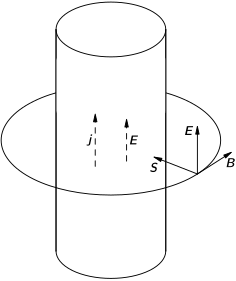
\includegraphics[width=1\linewidth]{FLC}
			\end{flushleft}
		\end{column}
		\begin{column}{0.7\linewidth}
			\begin{overprint}
				\onslide<1>
				\tiny
				Магнітне поле можна знайти з теореми про циркуляцію:
				\begin{equation*}
					B = \frac{2I}{cr},
				\end{equation*}
				де $ r $ --- радіус циліндра.
				Електричне поле знайдемо із закону Ома
				\begin{equation*}
					E = \frac{I\rho}{S} = \frac{IR}{\ell},
				\end{equation*}
				де $ \ell $ --- довжина частини провідника.

				Вектор Пойнтінга (енергія яка втікає в провідник за секунду в одиничну площу):
				\begin{equation*}
					S = \frac{c}{4\pi} E B = \frac{I^2R}{2\pi r \ell},
				\end{equation*}
				$ 2\pi r l $ --- площа бічної поверхні провідника на довжині $ \ell $.

				Повна потужність, яка втікає в провідник $ S\cdot 2\pi r \ell $, і дорівнює
				\begin{equation*}
					P = S\cdot 2\pi r \ell = I^2 R.
				\end{equation*}
				\onslide<2>
				\begin{block}\justifying\small
					Таким чином, електрони отримують свою енергію, ззовні, від потоку енергії зовнішнього поля всередину дроту і витрачають її на створення теплоти.

					\bigskip

					Енергія віддалених зарядів якимось чином розтікається по великій області простору і потім втікає всередину дроту.
				\end{block}
			\end{overprint}
		\end{column}
	\end{columns}

\end{frame}
% ===========================================================================



% ============================== Слайд ## ===================================
\begin{frame}{Файнман про енергію та імпульс поля}{\url{https://www.feynmanlectures.caltech.edu/II_27.html}}
	\begin{columns}
		\begin{column}{0.5\linewidth}
			\begin{center}
				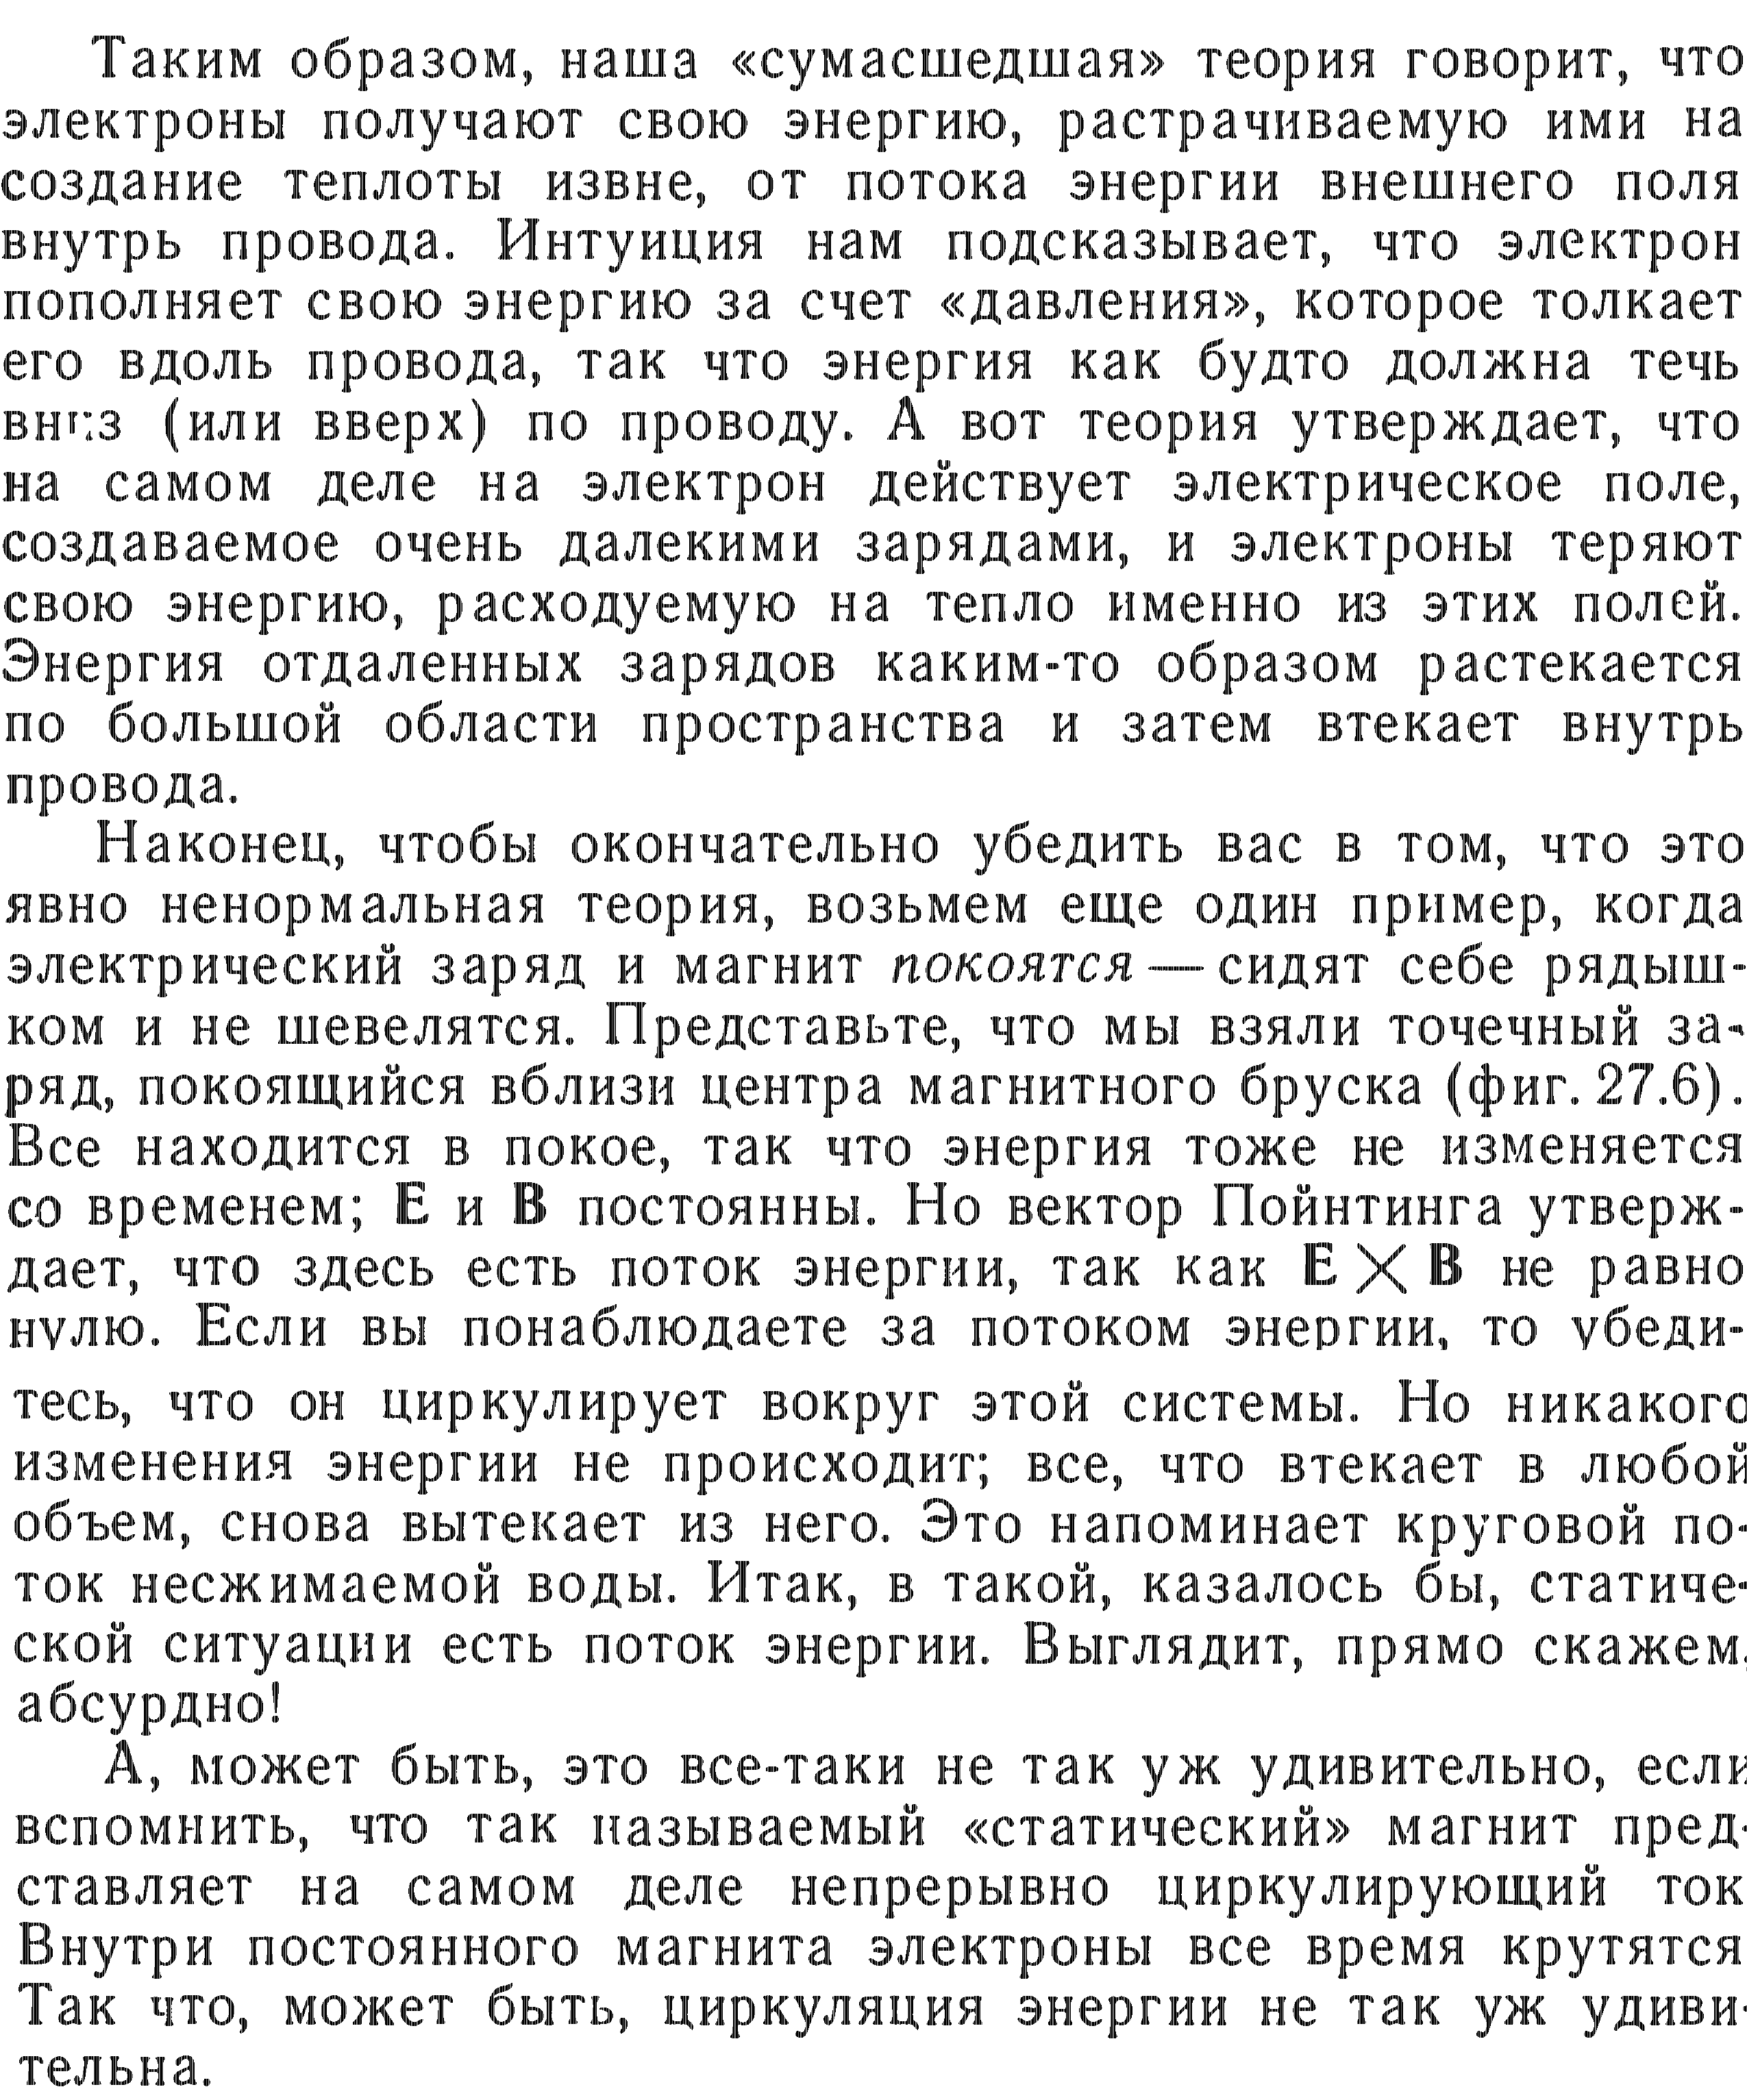
\includegraphics[width=1\linewidth]{FLMa}
			\end{center}
		\end{column}
		\begin{column}{0.5\linewidth}
			\begin{center}
				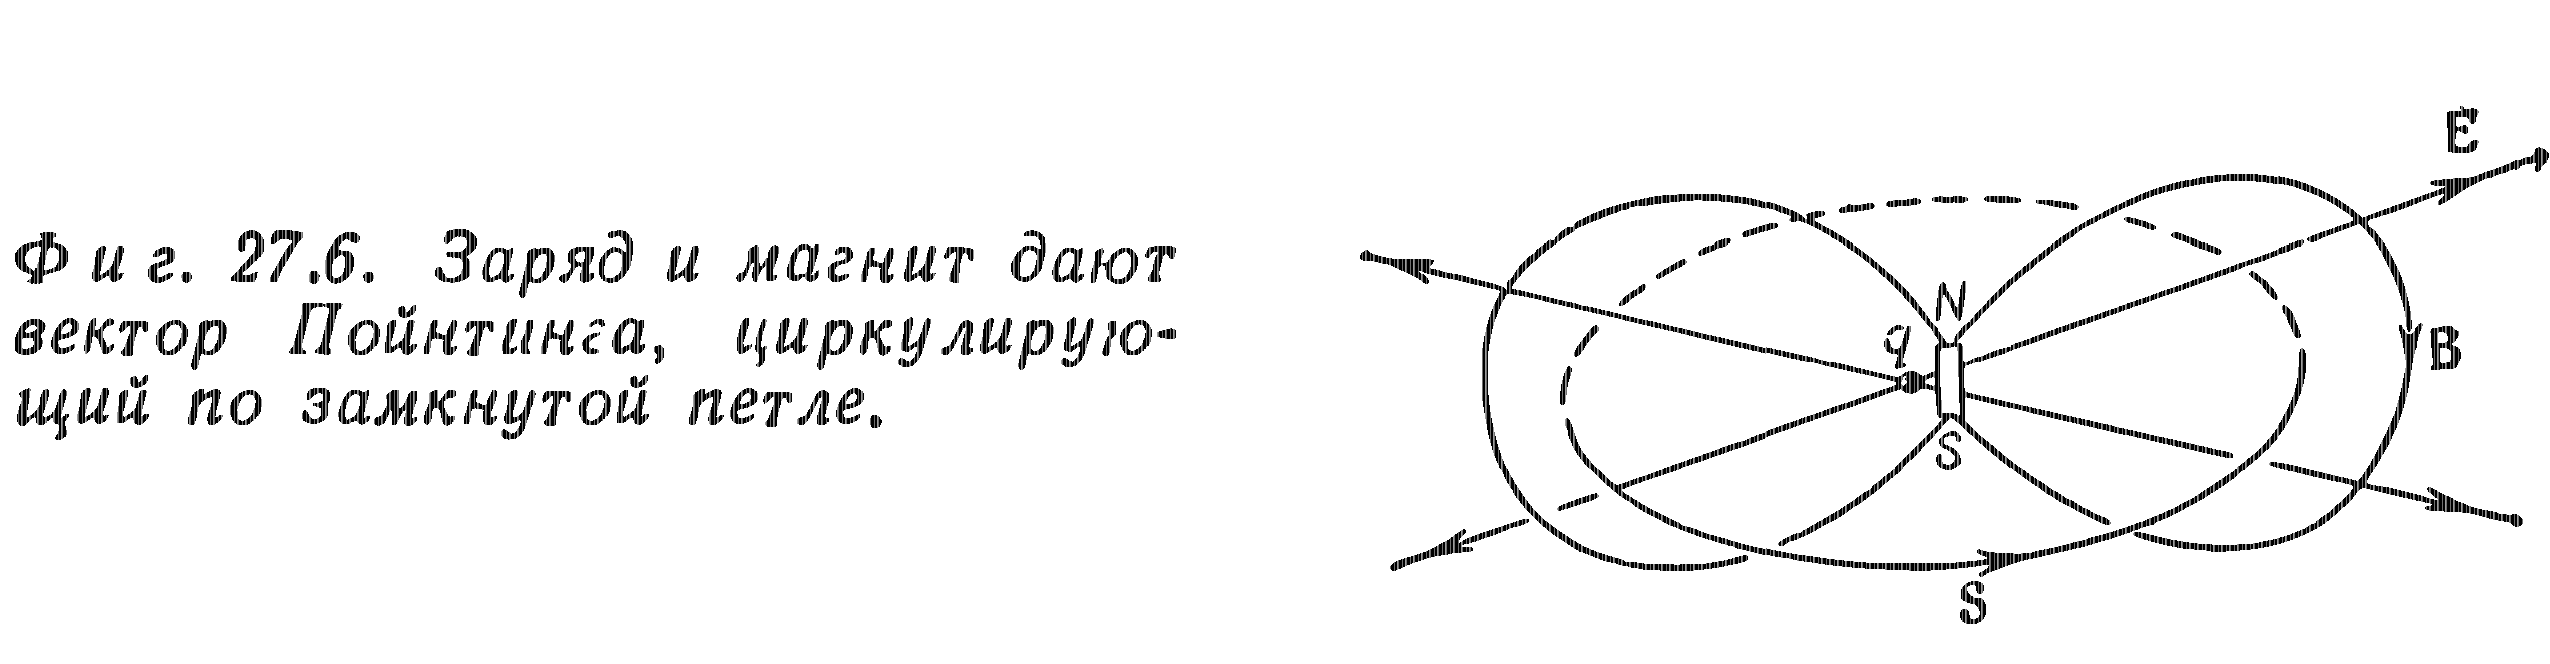
\includegraphics[width=1\linewidth]{FLMb}
			\end{center}
		\end{column}
	\end{columns}
	\vfill

	\begin{block}{}\tiny
		\url{https://youtu.be/6Hv2GLtnf2c}\\
		\url{https://youtu.be/D0TFS2Rb-vc}
	\end{block}
\end{frame}
% ===========================================================================



% =================================================
\begin{frame}[t]{Плоскі електромагнітні хвилі}
	\begin{onlyenv}<1-3>
		\begin{align}
			\vect{E} & = \vect{E}_m e^{i(\omega t - \vect{k}\vect{r})} \label{Ew} \\
			\vect{B} & = \vect{B}_m e^{i(\omega t - \vect{k}\vect{r})} \label{Bw}
		\end{align}
	\end{onlyenv}

	% -------------------------------------------------
	\begin{onlyenv}<1>

		\begin{center}
			\begin{tikzpicture}[scale=0.75]
				\clip (-1,-1) rectangle (6,5);
				\draw[->] (0, -1) to (0,5) node[below left] {$y$};
				\draw[->] (-1, 0) to (6,0) node[below left] {$x$};
				\foreach \i in {0,1,...,5} {
						‎\draw[domain=-1:30, smooth, variable=\x, blue] plot ({\x}, {-\x + \i}) ;
					}
				\coordinate (K) at (1.5, {-1.5 + 4});
				\draw[->] (0,0) -- node[left=1pt] {$\vect{r}$} (K);
				\draw[->, red, double] (K) -- ++(45:1) node[right] {$\vect{k}$};
			\end{tikzpicture}
		\end{center}
	\end{onlyenv}

	% -------------------------------------------------
	\begin{onlyenv}<2>
		% Electromagnetic wave - colored
		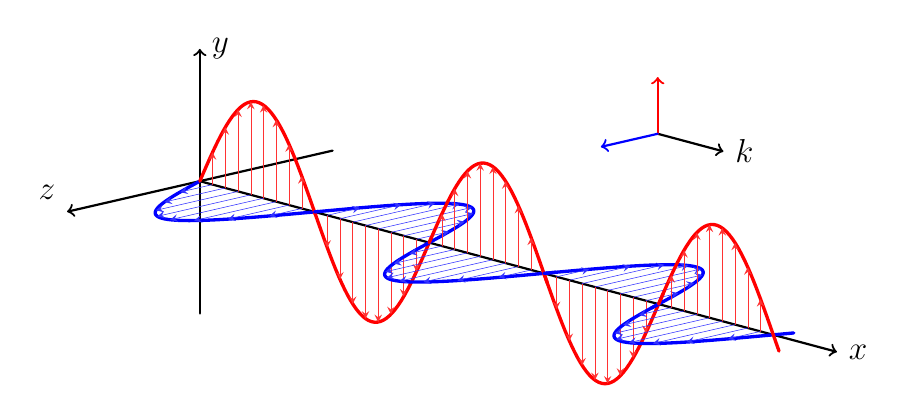
\begin{tikzpicture}[x=(-15:1.2), y=(90:1.0), z=(-150:1.0),
				line cap=round, line join=round,
				axis/.style={black, thick,->},
				vector/.style={>=stealth,->}, scale=0.8]
			\large
			\def\A{1.5}
			\def\nNodes{5} % use even number
			\def\nVectorsPerNode{8}
			\def\N{\nNodes*40}
			\def\xmax{\nNodes*pi/2*1.01}
			\pgfmathsetmacro\nVectors{(\nVectorsPerNode+1)*\nNodes}


			\def\drawENode{ % draw E node and vectors with some offset
				\draw[red,very thick,variable=\t,domain=\iOffset*pi/2:(\iOffset+1)*pi/2*1.01,samples=40]
				plot (\t,{\A*sin(\t*360/pi)},0);
				\foreach \k [evaluate={\t=\k*pi/2/(\nVectorsPerNode+1);
							\angle=\k*90/(\nVectorsPerNode+1);}]
				in {1,...,\nVectorsPerNode}{
						\draw[vector, help lines, red!80]  (\iOffset*pi/2+\t,0,0) -- ++(0,{\A*sin(2*\angle+\iOffset*180)},0);
					}
			}
			\def\drawBNode{ % draw B node and vectors with some offset
				\draw[blue,very thick,variable=\t,domain=\iOffset*pi/2:(\iOffset+1)*pi/2*1.01,samples=40]
				plot (\t,0,{\A*sin(\t*360/pi)});
				\foreach \k [evaluate={\t=\k*pi/2/(\nVectorsPerNode+1);
							\angle=\k*90/(\nVectorsPerNode+1);}]
				in {1,...,\nVectorsPerNode}{
						\draw[vector,help lines, blue!80]  (\iOffset*pi/2+\t,0,0) -- ++(0,0,{\A*sin(2*\angle+\iOffset*180)});
					}
			}

			% main axes
			\draw[axis] (0,0,0) -- ++(\xmax*1.1,0,0) node[right] {$x$};
			\draw[axis] (0,-\A*1.4,0) -- (0,\A*1.4,0) node[right] {$y$};
			\draw[axis] (0,0,-\A*1.4) -- (0,0,\A*1.4) node[above left] {$z$};

			% small axes
			\def\xOffset{{(\nNodes-2)*pi/2}}
			\def\yOffset{\A*1.2}
			\def\zOffset{\A*1.2}
			\draw[axis,black] (\xOffset,\yOffset,-\zOffset) -- ++(\A*0.6,0,0) node[right,align=center] {$\vect{k}$}; %\\propagation
			\draw[axis,red]  (\xOffset,\yOffset,-\zOffset) -- ++(0,\A*0.6,0) node[right] {$\Efield$};
			\draw[axis,blue]   (\xOffset,\yOffset,-\zOffset) -- ++(0,0,\A*0.6) node[above left] {$\Bfield$};

			% equation


			% draw (anti-)nodes
			\foreach \iNode [evaluate={\iOffset=\iNode-1;}] in {1,...,\nNodes}{
					\ifodd\iNode \drawBNode \drawENode % E overlaps B
					\else        \drawENode \drawBNode % B overlaps E
					\fi
				}

		\end{tikzpicture}
	\end{onlyenv}

	% -------------------------------------------------
	\begin{onlyenv}<3>

		Підставимо \eqref{Ew} та \eqref{Bw} в рівняння Максвелла. 		Диференціальні операції заміняються на:

		\begin{equation*}
			\vect{\nabla} \to -i\vect{k}, \quad \frac{\partial}{\partial t} \to i\omega
		\end{equation*}

		\begin{equation*}
			\vect{k}\times\Efield    =\frac\omega{c}  \Bfield,    \quad
			-\vect{k}\times \Hfield =  \frac\omega{c} \epsilon\Efield
			%    k^2 \Efield &= \frac{n^2}{c^2} \omega^2 \Efield, \quad k^2 = \frac{\omega^2}{v^2}
		\end{equation*}


		\begin{equation*}
			k =  \frac{\sqrt{\epsilon\mu}}{c} \omega = \frac{n}{c} \omega = \frac{\omega}{v}, \quad n E_m = B_m, \quad \sqrt{\epsilon} E_m = \sqrt{\mu} H_m
		\end{equation*}
	\end{onlyenv}

	% -------------------------------------------------
	\framesubtitle<4>{Енергія хвилі та вектор Пойнтінга}
	\begin{onlyenv}<4>
		\begin{equation*}
			\vect{k}\times\Efield    =\frac\omega{c}  \Bfield,    \quad
			-\vect{k}\times \Hfield =  \frac\omega{c} \epsilon\Efield
			%    k^2 \Efield &= \frac{n^2}{c^2} \omega^2 \Efield, \quad k^2 = \frac{\omega^2}{v^2}
		\end{equation*}


		\begin{equation*}
			k =  \frac{\sqrt{\epsilon\mu}}{c} \omega = \frac{n}{c} \omega = \frac{\omega}{v}, \quad n E_m = B_m, \quad \sqrt{\epsilon} E_m = \sqrt{\mu} H_m
		\end{equation*}
		Густина енергії (амплітуда)
		\begin{equation*}
			w_m = \frac{\epsilon E_m^2}{8\pi} + \frac{\mu H_m^2}{8\pi}, \quad  \sqrt{\frac{\epsilon}{\mu}} E_m = H_m, \quad w_m = \frac{\epsilon E_m^2}{4\pi} = \frac{\mu H_m^2}{4\pi}.
		\end{equation*}

		Вектор вектор Пойнтінга $ \vect{S} = \frac{c}{4\pi}[\Efield\times\Hfield] $:

		%        \begin{equation*}
		%            \Efield = - \frac{c}{\epsilon \omega} \vect{k}\times\Hfield
		%        \end{equation*}

		\begin{equation*}
			\vect{S} =  \frac{c^2}{4\pi\epsilon \omega} \Hfield\times\vect{k}\times\Hfield = \frac{c^2}{4\pi\epsilon \omega} H^2 \vect{k} =  \frac{c}{\omega} \frac{1}{\epsilon\mu}\left( \frac{\mu H^2}{4\pi}\right)   c \vect{k} = w \frac{c}{\sqrt{\epsilon\mu}} \frac{\vect{k}}{k}= w \vec{v}.
		\end{equation*}
	\end{onlyenv}
\end{frame}
% ============================== Слайд ## ===================================






% ============================== Слайд ## ===================================
\begin{frame}{Тиск світла}{}
	\begin{block}{}\justifying\small
		Максвел теоретично показав, що електромагнітні хвилі, відбиваючись чи поглинаючись тілами, на які  вони падають, чинять на них тиск. Цей тиск виникає внаслідок впливу магнітного поля хвилі на електричні струми, що збуджуються електричним полем тієї самої хвилі.
	\end{block}
    \vspace*{-1.25em}
	\begin{columns}
		\begin{column}{0.4\linewidth}
			\begin{center}
				\includegraphics[width=1\linewidth]{pictures/elmagpresure}
			\end{center}
		\end{column}
		\begin{column}{0.6\linewidth}
			\begin{block}{}\justifying\small
				Електричне поле хвилі збуджує електричний струм густиною $ \vect{j} = \sigma\Efield $ ($ \vect{F} = e\Efield $). Внаслідок цього на об'єму середовища діє сила Ампера $ d\vect{F} = \frac1c[\vect{j}\times\Bfield] dV$, спрямована убік поширення хвилі. Ця сила та викликає тиск електромагнітної хвилі.

                \medskip

				\begin{overprint}
                \onslide<1>
					У випадку поглинання вся енергія, яка падає за секунду на поверхню $wv dS$ тіла, перетворюється на теплову $ jE dV $:
					\begin{equation*}
						dF = \frac1c j \frac{c}{v}E = \frac1vjE = \frac1v wvdS = w dS,
					\end{equation*}
					звідки тиск $ p = \frac{dF}{dS} = w $
				\onslide<2>
					У випадку часткового відбивання, тиск дорівнює
					\begin{equation*}
						p = w (1 + \rho),
					\end{equation*}
					де $ \rho = 0 \ldots 1$ --- коефіцієнт відбивання.
				\end{overprint}
			\end{block}
		\end{column}
	\end{columns}
\end{frame}

\begin{frame}{Тиск світла}{Дослід Лебедєва}
	\begin{columns}
		\begin{column}{0.5\linewidth}\small\justifying
			Петро Миколайович Лебедєв в 1899 р. вперше виміряв світловий тиск. Він підвісив на тонкій нитці коромисло з парою крилець на кінцях: поверхня в одного з них була зачорненою, забезпечуючи майже повне поглинання, а в іншого --- дзеркальною, забезпечуючи повне відбивання. Підвіс з крильцями утворив чутливі крутильні терези, що поміщаються в посудину, повітря в якому було відкачано.
		\end{column}
		\begin{column}{0.5\linewidth}\centering
			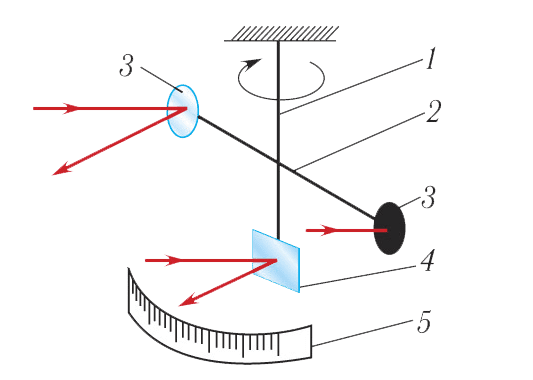
\includegraphics[width=\linewidth]{LebedevExp}
		\end{column}
	\end{columns}

	\begin{block}{}\small\justifying
		Світло практично повністю відбивалося від дзеркальної поверхні та його тиск на дзеркальне крильце було вдвічі більше, ніж на зачорнене. Внаслідок цього створювався момент сил, що повертає коромисло. Вимірюючи кут повороту коромисла, можна було виміряти силу, що діяла на крильця, а отже, визначити світловий тиск.
	\end{block}
	{\tiny \url{https://youtu.be/Dr07pTIoue8}}
\end{frame}

% ===========================================================================
\begin{frame}{Тиск світла}{Сонячні вітрила}
	\begin{onlyenv}<1>
		\begin{block}{}\small\justifying
			Сонячне вітрило --- пристрій, що використовує тиск сонячного світла чи лазера на дзеркальну поверхню для приведення в рух космічного апарату.

			\bigskip

			Тиск сонячного світла надзвичайно малий (на Земній орбіті --- близько $5\cdot10^{-6}$~Па) і зменшується пропорційно квадрату відстані від Сонця. В ролі вітрила використовувались сонячні батареї або радіатори системи терморегуляції.
		\end{block}

		\begin{center}
			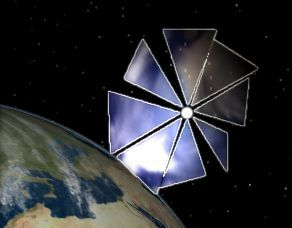
\includegraphics[width=0.4\linewidth]{Cosmos_solar_sail}
		\end{center}

		{\tiny \url{https://youtu.be/U0_wjnmlmRg}}
	\end{onlyenv}
	\begin{onlyenv}<2>
		\begin{block}{}\scriptsize\justifying
			Вчені з Австралійського національного університету запропонували спосіб запуску для космічного вітрильника до найближчої зірки Альфи Центавра в рамках проекту Breakthrough Starshot. За їх задумом, надати необхідну швидкість апарату допоможе фотонний двигун --- система, що сумарно включає до 100 мільйонів лазерів.
		\end{block}
		\begin{center}
			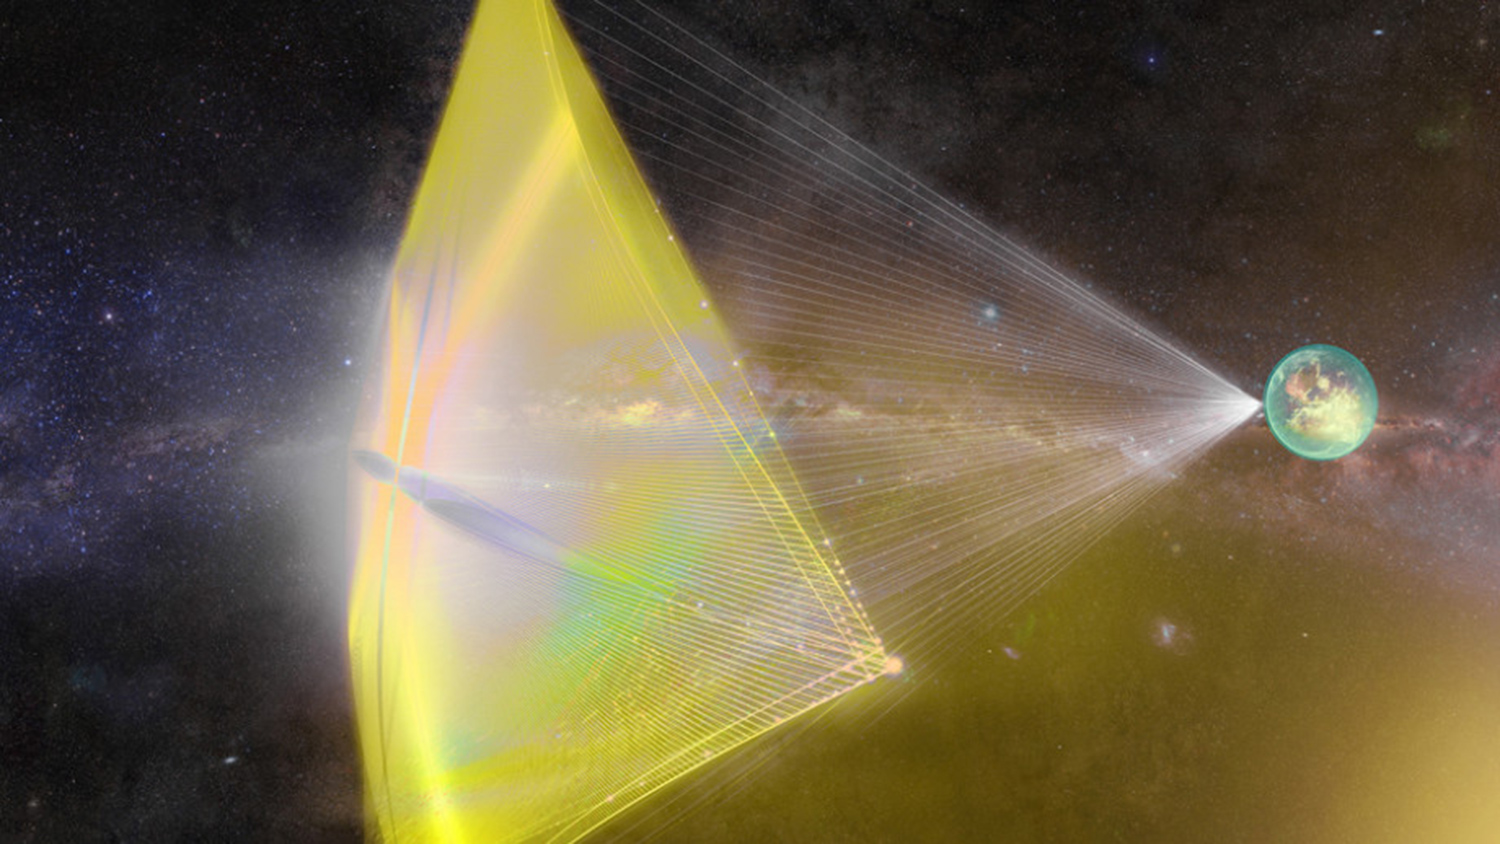
\includegraphics[width=0.5\linewidth]{Starshot-light-sail_Breakthroughinitiatives}
		\end{center}
		\begin{block}{}\scriptsize\justifying
			Подорож до Альфи Центавра за допомогою звичайних способів переміщення триватиме близько 100 років. Дістатись до Альфи Центавра за допомогою космічного вітрильника на фотонному двигуні передбачається за 20 років зі швидкістю в $ 0.2 c $.
		\end{block}
		{\tiny      \href{https://opg.optica.org/josab/fulltext.cfm?uri=josab-38-5-1477&id=450064}{Journal of the Optical Society of America B}.}
	\end{onlyenv}
	\begin{onlyenv}<3>
		\begin{block}{}\justifying\small
			Тиск світла відіграє велику роль в астрономічних та атомних явищах. В астрофізиці тиск світла поряд із тиском газу забезпечує стабільність зірок, протидіючи силам гравітації. Дія тиску світла пояснюються деякі форми кометних хвостів. До атомних ефектів відноситься так звана світлова віддача, яку відчуває збуджений атом під час випромінювання фотона.
		\end{block}
		\begin{columns}\centering
			\begin{column}{0.5\linewidth}\centering
				\includegraphics[width=\linewidth]{Star}
			\end{column}
			\begin{column}{0.5\linewidth}\centering
				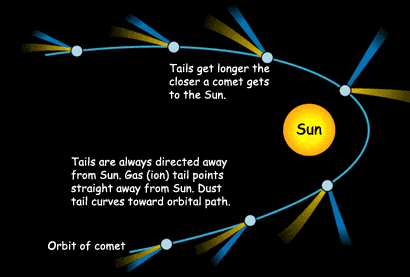
\includegraphics[width=\linewidth]{Comet}

				\begin{block}{}\tiny
					Товстий білий хвіст комети Гейла-Боппа складається з частинок пилу, і утворюється завдяки тиску світла. Другий, тонкий і блакитний складається з іонів і створюється сонячним вітром.
				\end{block}
			\end{column}
		\end{columns}
	\end{onlyenv}
\end{frame}
% ===========================================================================





% ============================== Слайд ## ===================================
\begin{frame}{Імпульс електромагнітного поля}{}
	\begin{block}{}\justifying\small
		Поле має енергію; так само в одиниці об'єму воно має якийсь імпульс. Оскільки електромагнітна хвиля чинить тиск на речовину, остання набуває певного імпульсу. Але в замкнутій системі, що складається з речовини та електромагнітної хвилі, виникло б порушення закону збереження імпульсу, якби імпульс мала лише речовина.
	\end{block}

	Для електромагнітної хвилі у вакуумі вектор Пойнтінга.
	\begin{equation*}
		S = w c \Rightarrow \frac{S}{c^2} = \frac{w}{c}.
	\end{equation*}

	З релятивістської механіки $ E^2 = m^2c^4 + p^2c^2 $. Для частинки з нульовою масою (наприклад, фотона) $ m = 0 $, зв'язок енергії та імпульсу:
	\begin{equation*}
		E = p c \Rightarrow  p = \frac{E}{c}.
	\end{equation*}

	Порівнюючи дві останні формули, отримаємо вираз для густини імпульсу:
	\begin{equation*}
		\vect{g} = \frac{\vect{S}}{c^2}, \quad [g] = \frac{\text{дин}\cdot\text{с}}{\text{см}^3}\, \text{(СГС)}
	\end{equation*}
\end{frame}
% ===========================================================================




% ============================== Слайд ## ===================================
\begin{frame}{Момент імпульсу поля}{}
	\begin{block}{}\scriptsize\justifying
		Заряджений циліндричний конденсатор вміщений в зовнішнє однорідне магнітне поле з індукцією $ \Bfield $, яке напрямлене вздовж його осі. Конденсатор має змогу вільно обертатись навколо своєї осі. Заряд конденсатора $ q $, радіус зовнішньої обкладки $ R $, радіусом внутрішньої можна знехтувати.  Маса конденсатора $ m $. Знайдіть вектор моменту імпульсу електромагнітного поля конденсатора. Знайдіть кутову швидкість, з якою буде обертатись конденсатор, при вимикання магнітного поля.
	\end{block}
	\begin{columns}
		\begin{column}{0.3\linewidth}
			\begin{center}
				\begin{tikzpicture}[scale=1.5]
					\draw [fill=gray, fill opacity=.25]
					(180:1mm) coordinate (a)
					-- ++(0,-15mm) coordinate (b)
					arc (180:360:1mm and 0.25mm) coordinate (d)
					-- (a -| d) coordinate (c) arc (0:180:1mm and 0.25mm);
					\draw [fill=gray, fill opacity=.25]
					(0,0) coordinate (t) circle (1mm and 0.25mm);
					\draw [densely dashed] (d) arc (0:180:1mm and 0.25mm);

					\draw [thick]
					(180:7.5mm) coordinate (A)
					-- ++(0,-15mm) coordinate (B) %node [midway, right, inner sep=1pt] {$v$}
					arc (180:360:7.5mm and 2.625mm) coordinate (D)
					-- (A -| D) coordinate (C) arc (0:180:7.5mm and 2.625mm);
					\draw [thick]
					(0,0) coordinate (T) circle (7.5mm and 2.625mm);
					\draw [densely dashed] (D) arc (0:180:7.5mm and 2.625mm);

					\foreach[count=\j] \i in {-0.5, 0, 0.5} {
							\draw[blue, <-] (\i,5mm) \ifnum\j=2 node[above] {$\Bfield$} \fi -- ++(0,-25mm);
						}

					\foreach[count=\j] \i in {0, -0.5, -1, -1.5} {
							\draw[red, ->] (1mm,\i) -- ++(6.5mm,0) \ifnum\j=2 node[right] {$ \Efield $}\fi;
							\draw[red, ->] (-1mm,\i) -- ++(-6.5mm,0);
						}

					\draw (0,0) ellipse (1mm and 0.25mm);

					\draw[green!50!black, <-] (0,-0.75) [partial ellipse=110:430:4mm and 1.3mm] node[above, pos=0.2] {$ \vect{S} $};

				\end{tikzpicture}
			\end{center}
		\end{column}
		\begin{column}{0.7\linewidth}\tiny
			Густина моменту імпульсу поля:
			\begin{equation*}
				\vec{\mathcal{L}} = \vect{r}\times\frac{\vect{S}}{c^2} = \frac{1}{4\pi c} \vect{r}\times \Efield \times \Bfield = - \frac{1}{4\pi c} \Bfield (\vect{r}\cdot \Efield)
			\end{equation*}

			Електричне поле можна визначити за формулою:
			\begin{equation*}
				E = \frac{2\lambda}{r} = \frac{2q}{rh}, \quad h - \text{висота циліндра}
			\end{equation*}

			Модуль вектора імпульсу $ \vect{L} $:
			\begin{equation*}
				L = \iiint\limits_V\mathcal{L} dV = \frac{1}{4\pi c} B \frac{2q}{h} \pi R^2 h = \frac{qBR^2}{2c}, \quad \vect{L} = - \frac{qR^2}{2c} \Bfield
			\end{equation*}
			При вимиканні магнітного поля момент імпульсу має зберегтися, тому він перейде в обертання самого циліндра $ \vect{L} = mR^2\vec\omega $, а тому кутова швидкість:
			\begin{equation*}
				\vec{\omega} = -\frac{q}{2mc}\vect{B}
			\end{equation*}
		\end{column}
	\end{columns}


\end{frame}
% ===========================================================================

\end{document}
